
\chapter{Technical Background and Disambiguation}
\label{cha:Disambiguation}
% [TODO] General info, introduction of chapter

\section{Intelligent Transportation Systems (ITS)}
Intelligent Transportation Systems (ITS) apply information and communication technologies to vehicles, transportation infrastructure and its users aiming to provide services to enhance road safety, mobility and traffic efficiency. % goals

% .... 


% ...ITS not only for road vehicles
Initially ITS have been only apparent in the road transport domain, yet began to appear in other domains such as in maritime and rail transport. % proof?
This development lead to expansion of ITS original ``Fundamental services'' which have been defined in the international standard ISO 141813-1 in 1999. % citation
With the most recent version (2016), ITS are now expected to address the following service domains:

% service domains (where each holds different service groups)
\begin{multicols}{2}
    \begin{itemize}
        \item Traveler information
        \item Traffic management\\and operations
        \item Vehicle services
        \item Freight transport
        \item Public transport
        \item Emergency
        \columnbreak
        \item Transport-related electronic\\payment
        \item Road transport-related\\personal safety
        \item Weather and environmental\\conditions monitoring
        \item Disaster response management\\and coordination
        \item National security.
    \end{itemize}
\end{multicols}

While ITS offer services to different domains, generally ITS services are about enhancing the driving experience. ITS can exist without intercommunication with other ITS or other vehicles, such as \textit{lane departure warning systems} and \textit{adaptive cruise control} that use technologies like video pattern recognition and radar to provide assistance to the driver. \cite{} % Intelligent Transport Systems Standards by Bob Williams

% Difference C-ITS vs ITS
% The main difference between C-ITS applications and conventional ITS applications is that C- ITS applications rely on common communication architecture between all connected entities allowing them to exchange all type of information

However, \textbf{Cooperative Intelligent Transportation Systems} (C-ITS) are the most promising technology to contribute to ``improving road safety by avoiding accidents and reducing their severity, to decreasing congestion, by optimising performance and available capacity of existing road transport infrastructure, to enhancing vehicle fleet management, by increasing travel time reliability and to reducing energy use and negative environmental impact''.
% EU - Deployment and Operation of European Cooperative Intelligent Transport Systems (C-ITS)
The emphasis of C-ITS lays on the term ``coperative'' which highlights the ability to communicate and share information with other vehicles and/or infrastructure, in order to increase their awareness about their surroundings.
To achieve this a proper, standardized communication architecture is required. In Europe, the European Telecommunication Standards Institute (ETSI) administers this process based on advisements by the Car-2-Car (C2C) Communication Consortium\footnote{Website Car-2-Car Communication Consortium: \url{https://car-2-car.org/}}.
The C2C consortium is compromised of leading vehicle manufacturers, equipment suppliers, research organizations and other partners who focus ``on creating standards ensuring the interoperability of cooperative systems spanning all vehicles classes, across borders and brands''\cite{}. % source flyer
C-ITS and a successful standardization process are necessary for the future of automated, driverless vehicles and their integration into the global transportation system.

ITS applications and services that utilize sensors are already an extensive contribution for vehicles themselves, yet their scope are even more auxiliary and beneficial for other proximate entities when applicable sensor information are shared using real-time messages.
Subsequently, a vehicular communication system has been developed during the ITS standardization process which allows the bidirectional message exchange between vehicles and any entity that may affect it.
Based on the vehicle's information exchange with other entities this communication is called ``Vehicle-to-everything'' (V2X) communication.

% mention diff. V2X technologies
The underlying technology of V2X communication creates a wireless connection between the communicating vehicle and entity, by either establishing a WiFi or cellular-based connection.

% TODO correct!!!
\textbf{In the United States this kind of WiFi-based connection is commonly referred to and has been standardized as 'dedicated short range connection' (DSRC), whereas in Europe an equivalent standard emerged and is named 'ITS-G5'.} Their cellular correspondent is called cellular V2X (C-V2X) communication and uses 3G, LTE or soon, with it's impending introduction, 5G networks.
A more in-depth look at mentioned V2X communication technologies is provided in section \ref{sec:v2xtech}.

% Transition to ITS Stations
ITS applications are distributed over several ITS stations, which interact together to satisfy a large diversity of services. % ETSI TS 102 637-1
Such ITS stations are equipped with multiple communication capabilities, which vary depending on the ITS station's type. The ETSI distinguishes between four different types of ITS stations: 
\begin{itemize}
    \item Central ITS station,
    \item Roadside ITS station,
    \item Vehicle ITS station and
    \item Personal ITS station.
\end{itemize}

% Central ITS station
\noindent A central ITS station is an organizational entity, which operates centrally managed ITS applications and services.
This includes traffic management centers that control and monitor roadside infrastructure, fleet management centers as well as any service or content provider that distributes information (via roadside components) to other ITS stations.

% connections
Central ITS station are known to have both a wireless and wired connection.
% -- wireless to communicate directly with ITS (uncommon)
The wireless connection is to communicate directly with vehicle ITS station

% -- wired connection
Whereas the wired connection is 
used to communicate with roadside units, but also with backend

Vehicles, or yet more commonly, roadside infrastructure components send information to the central component, which in return, may responds similarly by sending information back to vehicles or roadside infrastructure.

The information exchange is accomplished using 
This information exchange is achieved, transmitted,

Central ITS systems are not 
not limited by the spanned V2X network, yet might be connected to o

% -- wired (backend)
not necessarily a closed network system, yet it might be connect to
may include other backend systems and services to provide additional information.

It is a common occurrence that central ITS stations are connected to wired networks, to include backend systems and services, that are necessary to provide additional information.



additional information 
- weather information, road status: surfaces, traffic situation

send information via V2X technologies to ITS Station

% {example Central ITS station} ?
% service provider (parking system: free, occupied space; toll: payment)



% {Roadside ITS station}
%     - roadside (provides independently or cooperatively applications for central or other roadside ITS stations)

example roadside like ...
Road side ITS station (RSU) is installed on the motorway ramp to monitor road section on end of the ramp. The ITS station takes images from the road section with stereo camera and calculates road weather type with IcOR software developed by VTT

communicate with central or other roadside

located in the roadside infrastructure

% Vehicle ITS station
%     - vehicle (provides application for driver and/or passengers. may require access to vehicle system e.g. CAN)

Vehicle ITS station a mobile device can be seen as an additional HMI for the driver, passenger or codriver. In that case the mobile device acts as a display device echoing interface elements for the user. It displays icons, texts and plays audio tones triggered and is commanded by the Application Unit (AU).

communicate with other roadside or other vehicle

located in a vehicle

% Personal ITS station
%     - personal (provides application to personal and nomadic(?) devices)



% example ITS Stations (picture, description)

mesh network - VANET?

% {...}

% {Transition to ITS messaging}
% The communications are achieved through exchanged V2X messages using multiple communication protocol stacks as defined in [i.1]

% point-to-point: communication from an ITS station to another ITS station. This includes the point to point communication and point-to-point session between the two ITS stations;
% point-to-multipoint: communication from an ITS station to multiple ITS stations. 










% communication modes
% - point-to-point: communication from an ITS station to another ITS station.
% - point-to-multipoint: communication from an ITS station to multiple ITS stations. 


% Transition to ITS Messaging services and brief mentioning about message sets (
[ ITS messaging ]
% ETSI defines 2 basic messaging services (also known as facilities) in communication stack of ITS application:
    % coop. awareness basic service -> CAM
    % coop. environmental basic service -> DENM
% [more details explained in next section]



% [DATA ACQUISITION]
\newpage

\section{Vehicle-to-everything (V2X) communication}
\label{sec:v2x}
[TODO]

% Vehicular Communications (TS 102 637-1)
% https://www.etsi.org/deliver/etsi_ts/102600_102699/10263701/01.01.01_60/ts_10263701v010101p.pdf
% https://www.auto-talks.com/technology/dsrc-vs-c-v2x-2/
% https://www.auto-talks.com/wp-content/uploads/2018/09/Global-V2X-DSRC-and-C-V2X-whitepaper.pdf


% point-to-point: communication from an ITS station to another ITS station
%    (includes point-to-point communication and session between the two ITS station)
% point-to-multipoint: communication from an ITS station to multiple ITS stations. 


% Vehicle to Infrastructure (V2I)
% Vehicle to Vehicle (V2V)
% Vehicle to Pedestrian (V2P)
% Vehicle to Network (V2N)

\newpage

\section{V2X Technologies}
\label{sec:v2xtech}
% [TODO] about V2X Technologies (Wireless communication protocols)

% formed network is called 'VANET' for Vehicular Adhoc Network
% in 5GHz spectrum

% xxx for US    - 5.9 GHz
% ETSI for EU   - 5.9 GHz
% AIRB for JP   - 5.*8* GHz

\subsection{Dedicated Short Range Communications (DSRC)}
% foundation is IEEE 802.11p, commonly referred to as wireless access in vehicular environment (WAVE)
% IEEE 802.11p is a modification of 802.11a
% frequency band is in 5.9GHz spectrum

% Tab.: Differences 802.11 *p* and *a*
\begin{table}[H]
    \centering
    \begin{tabular}{|l|c|c|l|}
        \hline
        \textbf{Parameters} & \textbf{IEEE 802.11a}  & \textbf{ IEEE 802.11p} & \textbf{Changes} \\ \hhline{====}
        Frequency Band      & 5/2.4 GHz     & 5.9 GHz           & two times \\ \hline
        Channel Bandwidth   & 20 MHz        & 10 MHz            & half \\ \hline
        Bitrate Mb/s &
        \begin{tabular}[c]{@{}c@{}}
            6, 9, 12, 18,\\
            24, 36, 48, 54
            \end{tabular}
        &
            \begin{tabular}[c]{@{}c@{}}
                3, 4.5, 6, 9,\\
                12, 18, 24, 27
            \end{tabular}
        & half \\ \hline
        Modulation & \multicolumn{2}{c|}{
            \begin{tabular}[c]{@{}c@{}}
                BPSK, QPSK,\\
                16-QAM, 64-QAM
            \end{tabular}}
        & no change \\ \hline
        Channel coding      & \multicolumn{2}{c|}{1/2, 1/3, 1/4}    & no change \\ \hline
        No. of subcarriers  & \multicolumn{2}{c|}{52}               & no change \\ \hline
        Subcarrier spacing  & 0.3125 MHz    & 0.15625 MHz           & half \\ \hline
        Symbol interval     & 4 $\mu s$     & 8 $\mu s$             & two times \\ \hline
        Guard time          & 0.8 $\mu s$   & 1.6 $\mu s$           & two times \\ \hline
        FFT Period          & 3.2 $\mu s$   & 6.4 $\mu s$           & two times \\ \hline
        Preamble duration   & 16 $\mu s$    & 32 $\mu s$            & two times \\ \hline
    \end{tabular}
    \caption{meaningful caption of table}
    \label{tab:802.11pa-table}
\end{table}

uses orthogonal frequency-division multiplexing (OFDM)
communication range: up to 1000m
channel bandwidth: [10, 20] MHz

% Fig.: 802.11p (WAVE) Channel Freq. 
\begin{figure}[H]
    \centering
    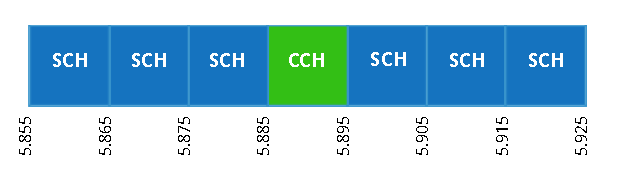
\includegraphics[
        width=0.7\textwidth
    ]{802-11p-spectrum.pdf}
    \caption{Frequency allocation of IEEE 802.11p in the US}
    \label{fig:802-11p-spectrum}
\end{figure}

% List: Channel types
\begin{enumerate}
    \item SCH1: (5.875 - 5.885 GHz) will be used for safety messages with lower priority (in comparison with CCH) and traffic efficiency applications.
    \item SCH2: (5.895 - 5.905 GHz) will be used for short distance transmissions which results in lower interference for SCH1 and CCH, because of the lower transmit power.
    \item CCH: (5.885 - 5.895 GHz) will be used for high priority safety messages and beacons.
\end{enumerate}

% --- WAVE OSI layers
% Fig. WAVE/DSRC Protocol Stack/OSI layers
\begin{figure}[H]
    \centering
    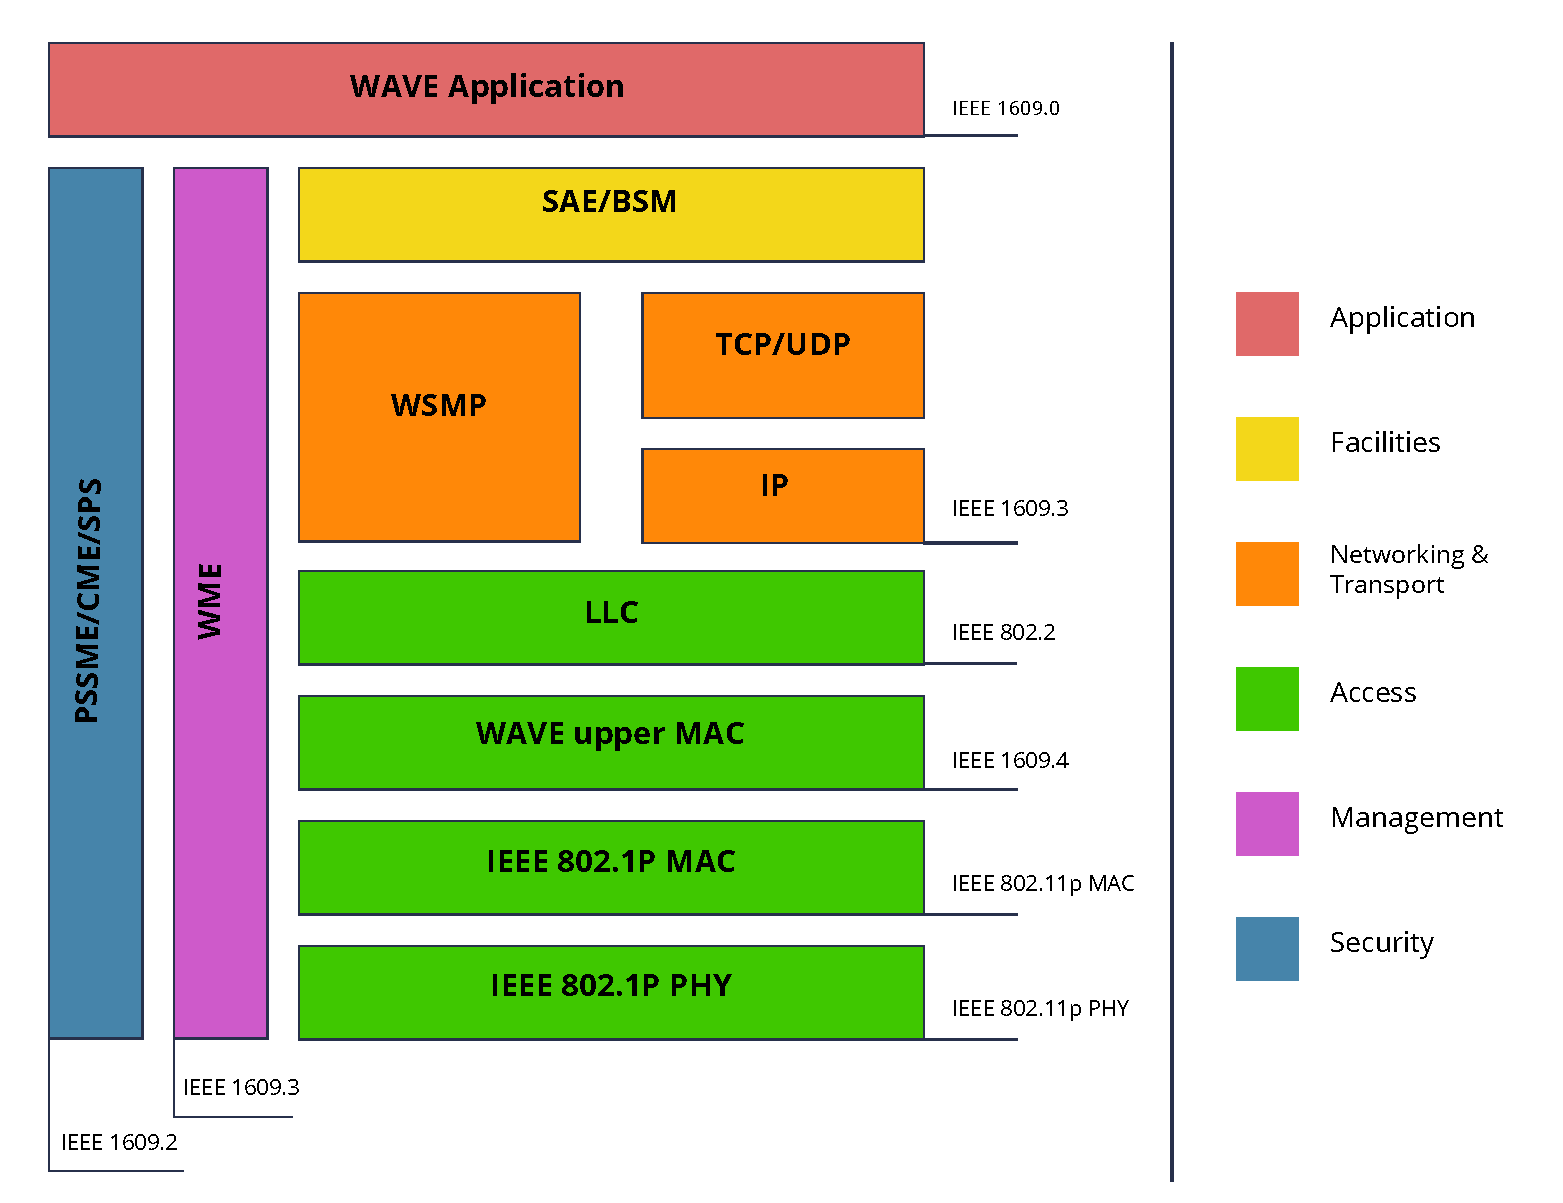
\includegraphics[
        width=\textwidth
    ]{WAVE-IEEE-1609.pdf}
    \caption{WAVE/DSRC protocol stack}
    \label{fig:iso-ieee-wave}
\end{figure}

% (OSI upper MAC layer) - IEEE 1609.4
% Multichannel operation -> 1x Control channel (CCH), 6x Service channel (SCH)

% (OSI Transport? layer) - IEEE 1609.3
% WAVE short message protocol (WSMP)

% (OSI Security layer) - IEEE 1609.2
% provides authentication and optional encryption of DSRC messages based on digital signatures and certificates. To protect the privacy of drivers, certificates don’t contain information about the driver. What’s more, a vehicle uses a certificate only for a limited time, changing it frequently to make tracking more difficult.

% Message Dictionary (OSI Facility layer)
% SAE J2735 - Basic Safety Message (BSM)
%   ~ 300 bits, max. 10Hz
%   beacon messages, vehicle state information
% SAE J2945.1) - -?-

% example DSRC application (OSI Application layer)
% DSRC main goals

\newpage

\subsection{Cooperative Intelligent Transport Systems (C-ITS)}
% 802.11p for Europe is termed 'ITS-G5' by ETSI, which is derived from IEEE standard.
% ITS-G5 is standardized as ETSI EN 302 663.

% mention similarities/differences of 802.11p and ITS-G5

5.725 GHz - 5.875 GHz
OFDM

% Fig.: ITS-G5 channel frequency spectrum]
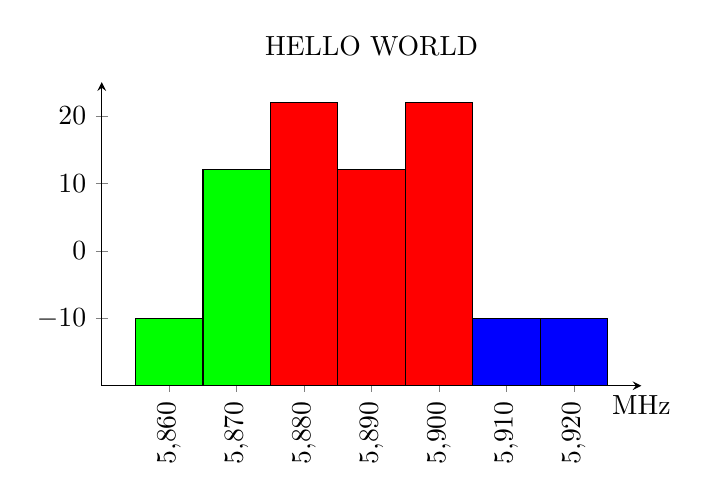
\begin{tikzpicture}
    \centering
    \begin{axis}[
        title=HELLO WORLD,
        xlabel=MHz,
        % https://tex.stackexchange.com/a/142121
        % ylabel near ticks,
        % xlabel near ticks,
        x label style={
            at={(axis description cs: 1, 0)},
            anchor=north
        },
        % ylabel={dBm/MHz},
        y label style={
            at={(axis description cs: 0, 1)},
            % rotate=270,
            anchor=south
        },
        xmin=5850, xmax=5930,
        ymin=-20, ymax=25,
        x tick label style={rotate=90},
        xtick={5860, 5870, 5880, 5890, 5900, 5910, 5920},
        ytick={-10, 0, 10, 20},
        axis x line=bottom, axis y line=left,
        axis equal image
        % axis line thick
    ]
    \draw [fill=green]  (axis cs:5855,-20) rectangle (axis cs:5865,-10); %SCH4
    \draw [fill=green]  (axis cs:5865,-20) rectangle (axis cs:5875, 12); %SCH3
    \draw [fill=red]    (axis cs:5875,-20) rectangle (axis cs:5885, 22); %SCH1
    \draw [fill=red]    (axis cs:5885,-20) rectangle (axis cs:5895, 12); %SCH2
    \draw [fill=red]    (axis cs:5895,-20) rectangle (axis cs:5905, 22); %CCH
    \draw [fill=blue]   (axis cs:5905,-20) rectangle (axis cs:5915,-10); %SCH5
    \draw [fill=blue]   (axis cs:5915,-20) rectangle (axis cs:5925,-10); %SCH6
    
    \end{axis}
\end{tikzpicture}

% ITS-G5 A (road safety related applications)
    % 30 MHz
% ITS-G5 B (non-safety application -> traffic efficiency)
    % 20 MHz
% ITS-G5 D (future ITS applications)
% divided into several channel bands of 10MHz frequency
% to avoid interference between channels and neighboring frequency bands, for each channel the per MHz power density is limited to -10dBm, 13dBm and 23dBm

% explain C-Band
% ITS-G5 C
    % operations also referred to
    % - broadband radio access networks (BRAN),
    % - radio local area network (RLAN)
    % and wireless local area network (WLAN)

% compare EU spectrum with US (it's compatible), (possibly) mention briefly incompatibility with Japan

% Fig.: C-ITS Protocol Stack/OSI layers
\begin{figure}[H]
    \centering
    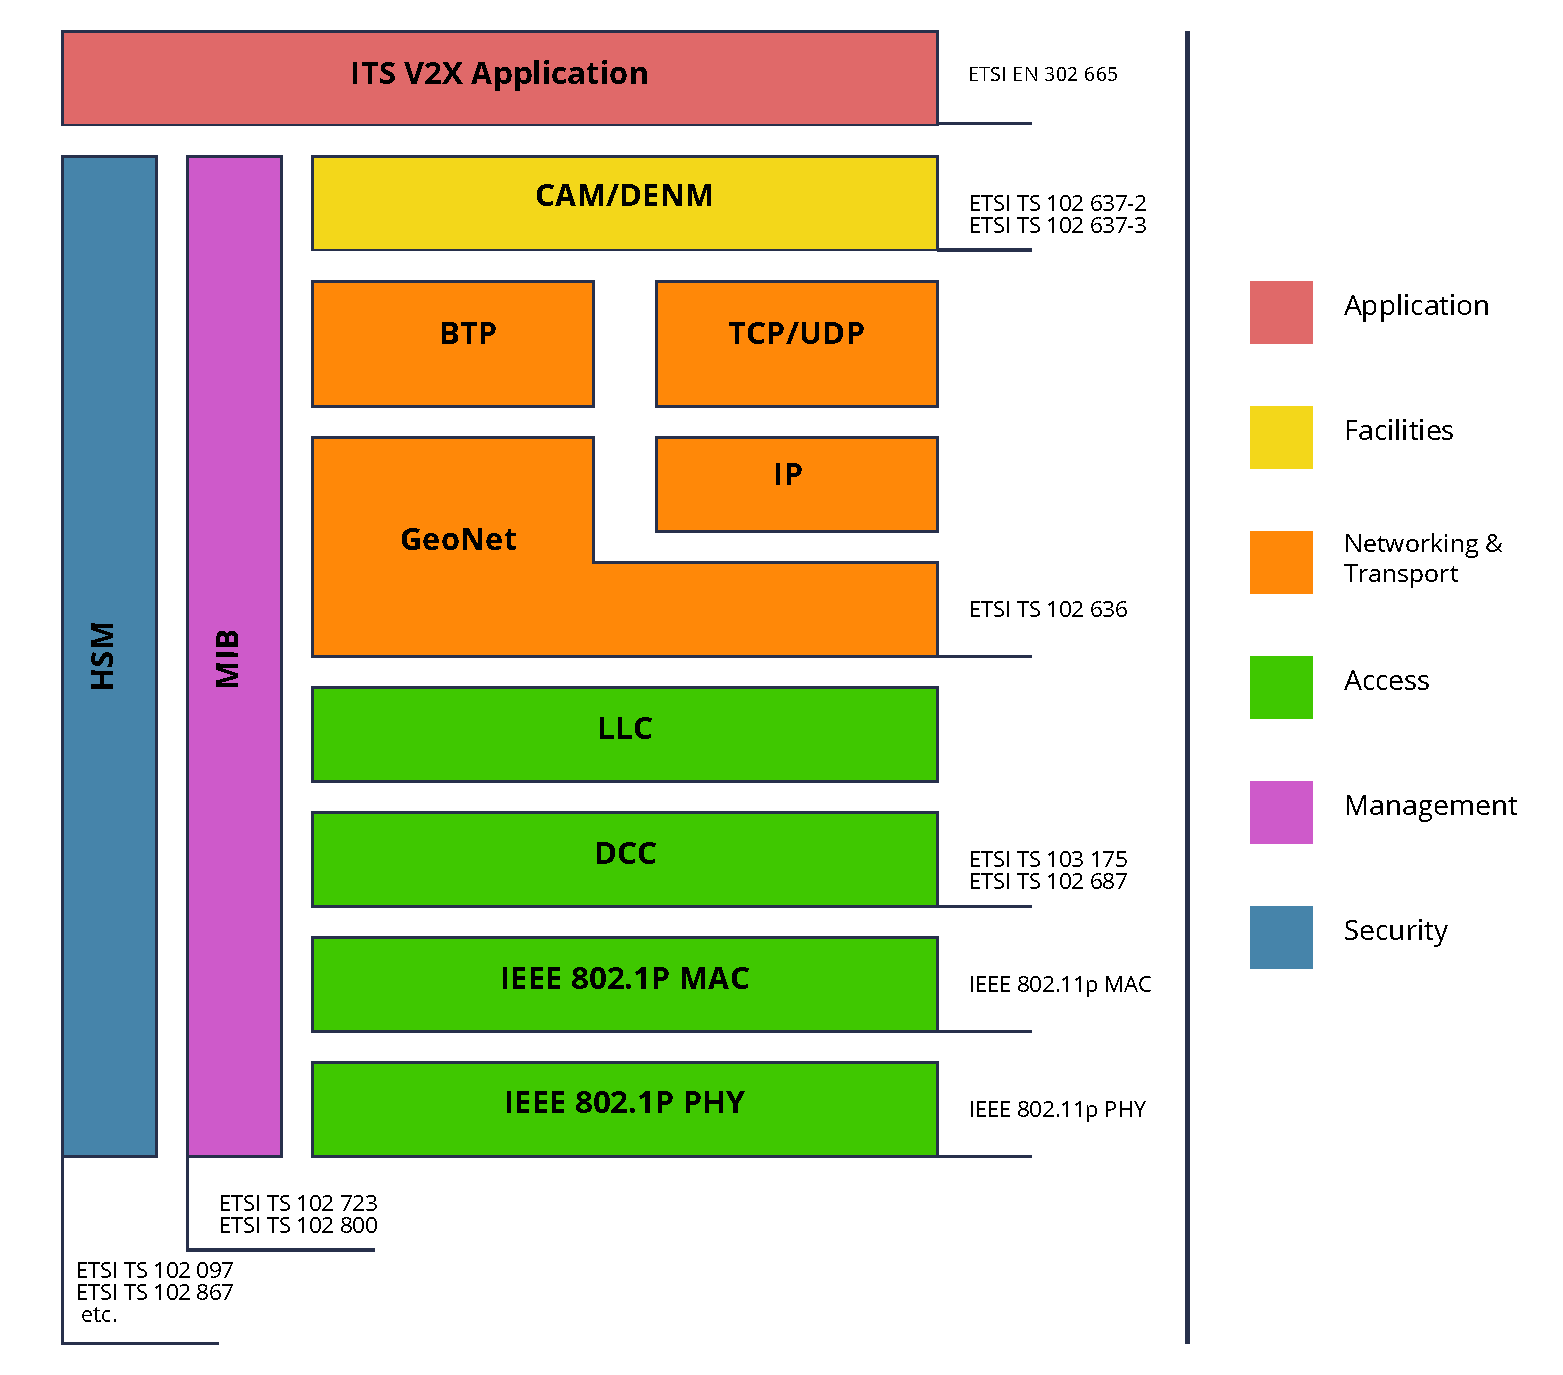
\includegraphics[
        width=\textwidth
    ]{ITS-G5.pdf}
    \caption{meaningful Caption about ITS-G5}
    \label{fig:iso-its-g5}
\end{figure}


% Message Dictionary Set (OSI Facility layer)
% EN 302 637-2 (CAM)
% EN 302 637-3 (DENM)

% example C-TIS application (OSI Application layer)

\subsection{Cellular-V2X (C-V2X)}
% V2X via LTE (or, future: 5G)
[TODO]
% ETSI TS 122 185 (maybe more)
% US ????

% src:
% https://ec.europa.eu/transport/sites/transport/files/themes/its/doc/c-its-platform-final-report-january-2016.pdf

\newpage

\section{V2X Message Sets}
% [TODO] General info, introduction to Message sets

V2X communication is the foundation of information exchange between ITS stations.


The foundation of 
For a successful

The information exchange of 


vehicular safety and traffic efficiency applications

needing continuous status information about surrounding vehicles and as



V2X communication
ITS applications

relevant information is wrapped in C2X Messages and transmitted by means of wireless communication


ETSI has defined 2 basic messaging services/2 facilities:
    - Cooperative Awareness Basic Service
    - Decentralized Environmental Notification Basic Service
    
periodic status exchange
asynchronous notifications

\subsection{Cooperative Awareness Messages (CAM)}
% ETSI EN 302 637-2
% use cases, in which applications there used

The CA basic service is a facilities layer entity that operates the CAM protocol. It provides two services: sending and receiving of CAMs.

notify presence of vehicle/road side station

CAM contains status and attribute information of the originating ITS-S.
The content varies depending on the type of the ITS-S.
information includes data about the dimensions, vehicle type and role in the road traffic, etc.


% CAM generation specs:
CAMs are generated periodically 
CAM generation frequency: 100 - 1000 ms (or 1-10Hz)
depending on dynamics and the channel congestion status

sent single hop
direct communication range.

CAM generation time shall be less than 50ms

new CAM must only be generated if the state has changed significantly


with received CAM calculate a local dynamic traffic map (LDM)


information about (at a specific time):
    geographic position
    speed
    driving direction (heading)

incl. confidence levels of
    heading,
    speed,
    acceleration
    curvature
    yaw rate
    length+width (precision of 10cm)

CAM's integrity and authenticity assured by signature and appropriate certificate
reveiver verifys message and temp validate (temporary freshness) it

% CAM size
CAM size                = ~2 KBit   (w/o special container)

header + Signature      =  750 bits
Base + HF + LF          =  200 bits
certificate             = 1000 bits
                         (1950 bits)

% explain cam structure, its containers and each field
Header:
    version
    message id
    generation time(stamp)
Basic: (mandatory)
    station type
    latest geographic position
    
HF: (mandatory)
    fast-changing (dynamic) status information -> heading and speed
    
    updated with every CAM
    
LF: (optional)
    static or slow-changing data  -> i.e. status of exterior lights

    no need of frequent update/not with every CAM

Special Vehicle: (optional)
    e.g. public transport, road works, emergency vehicles
    
    contains additional vehicle specific (state) information


% applications/use cases:
(in general: safety applications)

cooperative collision avoidance
slow vehicle warning
intersection collision warning
motorcycle approaching indication

remote vehicle monitoring
emergency vehicle warning


% Fig.: CAM table
\begin{figure}[H]
    \centering
    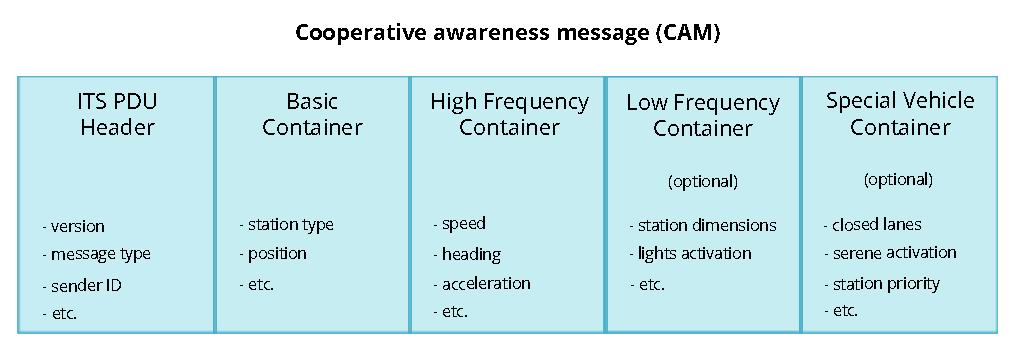
\includegraphics[
        width=\textwidth
    ]{CAM.pdf}
    \caption{Meaningful Caption CAM}
    \label{fig:cam-structure}
\end{figure}

\subsection{Decentralized Environmental Notification Messages (DENM)}
% ETSI EN 302 637-3

The DENM format is presented in Abstract Syntax Notation One (ASN.1).
Unaligned packed encoding rules (PER) shall be used for DENM encoding and decoding


event-driven

contains information about a specific dangerous, safety situation

notification may be generated from proximate road side unit, vehicles or from central station


on event status change the ITS application informs DENM facility to modify DENM message accordingly.

transmission of DENMs are either explicitly canceled (by its station) or get stopped since expiration time is reached







multi-hop/hop-by-hop techniques, forwarded by several hops
messages are repeated by multiple receiving stations
no specific destination, geocast mechanism 
    -> messages are forwarded towards geographical destination (store \& forward)
        or if already inside location, kept alive until end of their validity duration

% explain DENM structure, its containers and each field

% containers
header (same like CAM)
    version
    message id
    generation time(stamp)
Management (mandatory)
    [general information about event]
    
    message no.???

    actionID (refers to situation)
    
    time of detection
    station type/identifier
    event position
    
    validity duration/expiration time    (how long the msg is repeated)
    transmission frequency
Situation: (optional)
    [specific event details]
    information quality ( -> reliability of info, value 0 to X)
        severity?? (informative, obstacles, danger, highest danger)
    event type
    linkedCause
    eventHistory
    

Location: (optional)
    supplementing localization information, especially for moving situations
    
    event speed
    event position heading
    % situation position (concrete or geographical area)
    roadType    

A la carte: (optional)
    additional, use-case specific, information that is not provided by other containers.
    all provided information is optional
    
    lanePosition
    externalTempertature
    roadWorks
    positioningSolution
    stationaryVehicle

% Fig.: DENM table
\begin{figure}[H]
    \centering
    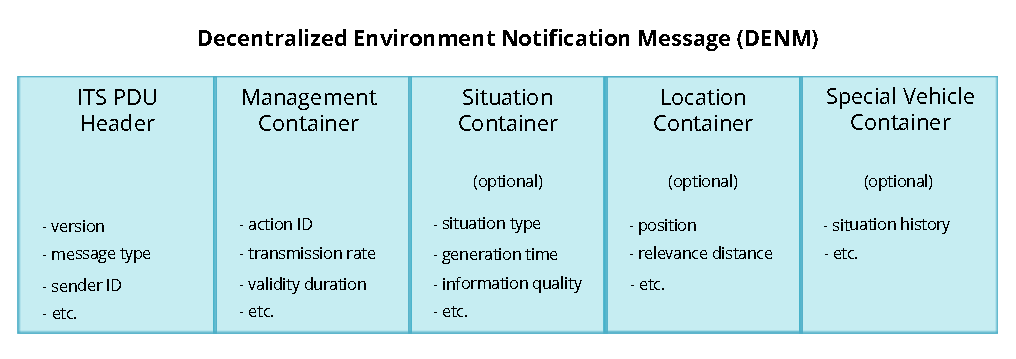
\includegraphics[
        width=\textwidth
    ]{DENM.pdf}
    \caption{meaningful caption DENM}
    \label{fig:denm-structure}
\end{figure}


% use cases, in which applications there used
Road Works Warning
Damaged Vehicle Warning
Emergency Electronic Brake Light
Traffic Jam Ahead Warning
Weather Hazard Warning

